%\documentclass[conference]{IAENGtran}
%\documentclass{sig-alternate}
\documentclass[a4paper, conference]{IEEEtran}
\usepackage{latexsym}
\usepackage{amssymb}
\usepackage{amsmath}
\usepackage{graphics}
%\usepackage[pdftex]{graphicx}
\usepackage{epsfig}
%\usepackage{calc}
%\usepackage{subfig}
%\usepackage{here}
%\usepackage{my}
\usepackage{ifpdf}
%\ifpdf
%\usepackage[pdftex]{graphicx}
%\usepackage[pdftex]{thumbpdf}      % Vignettes
%\usepackage[pdftex]{hyperref}      % Utilisation de HyperTeX
% \hypersetup{%
% %  bookmarks         = true,%       % Signets
%   bookmarksnumbered = true,%       % Signets num\'erot\'es
%   bookmarksopen     = true,%       % Affichage des signets.
%   pdfpagemode       = UseNone,%    % Signets/vignettes ferm\'e \`a l'ouverture
%   pdfborder         = {0 0 0},%    % Style de bordure : ici, pas de bordure
%   pdfstartview      = FitH,%       % La page prend toute la largeur
%   pdfpagelayout     = SinglePage,% % Vue par page
%   colorlinks        = true,%       % Liens en couleur
%   urlcolor          = blue,%       % Couleur des liens externes
%   linkcolor         = blue,%       % Couleur des liens externes
% %  pagecolor         = blue,%       % Couleur des liens externes
%   anchorcolor       = blue,%       % Couleur des liens externes
%   citecolor         = blue,%
%   filecolor         = blue,%
%   linktocpage       = true,%
%   breaklinks        = true,%       % retour ligne des liens trop longs
% %  backref           = true,%       % permet d'ajouter des liens dans...
% %  pagebackref       = true,%.      % ..les bibliographies
% %  hyperindex        = true,%       % ajoute des liens dans les index.
%   pdftitle    = {IAENG journal}
% }
%\DeclareGraphicsRule{*}{mps}{*}{}
% \else
% \usepackage[dvips]{graphicx}
% \usepackage[dvips]{hyperref}
% \fi

\usepackage{cite}
%\usepackage[pdftex]{color}
\usepackage{alltt}
\usepackage{url}
\usepackage{xspace}


% \pagestyle{plain} % remove before submission (numbered pages)
% \thispagestyle{empty}
% \pagestyle{empty}
%\IEEEoverridecommandlockouts


\newcommand{\hcinv}{\texttt{hc\_inversion}\xspace}
\newcommand{\inversion}{\coqdockw{inversion}\xspace}
\newcommand{\inv}{\coqdockw{inv}\xspace}
\newcommand{\simlight}{\texttt{Simlight}\xspace}
\newcommand{\compcert}{\texttt{CompCert}\xspace}
\newcommand{\clight}{\texttt{Clight}\xspace}
\newcommand{\simsoc}{\texttt{SimSoC}\xspace}
\newcommand{\simsoccert}{\texttt{SimSoC-Cert}\xspace}
\newcommand{\stt}{\small\tt}
\newcommand{\compcert}{Compcert\xspace}
\newcommand{\why}{\texttt{Why}\xspace}
\newcommand{\whyML}{\texttt{WhyML}\xspace}
\newcommand{\whyCert}{\texttt{WhyCert}\xspace}
\newcommand{\framac}{\texttt{Frama-C}\xspace}

\begin{document}

\title{Towards Certified Program Execution}

\author{ Vania Joloboff$^1$, Jean-Francois Monin$^2$,, Xiaomu
  Shi,$^2$}
\thanks{$^1$INRIA International FORMES project, and
  Shenzhen Institutes of Advanced Technology, Chinese Academy of
  Sciences, China, vania.joloboff@inria.fr}
\thanks{$^2$University of Grenoble, International FORMES project, China,
 [jean-francois.monin, xiaomu.shi]@imag.fr}
\maketitle

\pagestyle{empty}
\thispagestyle{empty}

\begin{abstract}
bla
\end{abstract}

%\IEEEkeywords{}


%%%%%%%%%%%%%%%%%%%%%%%%%%%%%%%%%%%%%%%%%%%%%%%%%%%%%%%%%%%%%%%%%%%%%%%%%%%%%
\section{Introduction} % => To be written by Vania or Claude
% introduction+abstract+title => 1+1/2 columns

It has long been a goal to exhibit a proof of program to certify that the
execution of a given algorithm is correct on the specific computer architecture
on which the program is executed. In particular in the area of cryptography
it is interesting to be confident that the resulting encrypted data output
by the computer is indeed the same as the result obtained with the formal
method describing by the algorithm.

Obtaining such certification is not a one step proof, it consists in a
series of steps requiring a tool chain. In this paper, we present an
attempt towards such a certification chain. Our approach towards this
certification of programs is the following.  Given the formal
specification of an algorithm, for example the AES cryptographic
encryption technique, one can derive a C program using formal or semi
formal methods such as B \cite{abrial-1996} or SCR
\cite{rothamel-2006} or \cite{apts-2008}.  In this paper we assume
that this phase has been achieved, that there is an existing C source
code program that is a provably correct implementation of the
specification. Our purpose is to show how it can be certified that the
execution of that C program on a given target architecture indeed
produces the expected results.  This requires the sequential following
steps, proving that (a) the translation from C to machine code and (b)
next the execution of the machine code are correct, that is, they
preserve the semantics of the source code.

The technique presented here relies largely on already existing tools,
in particular the Coq proof assistant, and the Compcert C compiler, a
certified compiler for the C language, combined with our own work to prove
the correctness of an ARM instruction set simulator.

The sequel of the paper presents the background existing tools,
related work, our method to combine these tools and our additional work
to reach the objectives.


%%%%%%%%%%%%%%%%%%%%%%%%%%%%%%%%%%%%%%%%%%%%%%%%%%%%%%%%%%%%%%%%%%%%%%%%%%%%%
\section{Related Work}
\label{related}

Program certification has to be based on a formal model of the program
under study.  Such a formal model is itself derived from a formal
semantics of the programming language.  Formal semantics are important
because they provide an abstract, mathematical, and standard
interpretation of a programming language.  There are three traditional
ways to express how programs perform computations: axiomatic
semantics, denotational semantics, and operational semantics.

Denotational semantics \cite{stoy-denotational} constructs
mathematical objects which describe the meaning of expressions of the
language using stateless partial \emph{functions}.  All observably
distinct programs have distinct denotations.  \

Axiomatic semantics and Hoare logic\cite{Floyd67, Hoare-1969} have
been widely used for proving the correctness of programs.  For
imperative programming languages such as C, a possible approach is to
consider tools based on axiomatic semantics, like
\framac~\cite{canet2009value}, a framework for a set of interoperable
program analyzers for C. Most of the modules integrated inside rely on
ACSL (ANSI/ISO C Specification Language), a specification language
based on an axiomatic semantics for C.  ACSL is powerful enough to
express axiomatizations directly at the level of the C program.  State
labels can be defined to denote a program control point, and can then
be used in logic functions and predicates.

\framac software leverages off from \why technology
\cite{bobot2011why3, filliatre07cav}, a platform for deductive program
verification, which is an implementation of Dijkstra's calculus of
weakest preconditions.  \why compiles annotated C code into an
intermediate language.  The result is given as input to the VC
(Verification Conditions) generator, which produces formulas to be
sent to both automatic provers or interactive provers like Coq.


Paolo Herms's \cite{herms13phd}~\cite{herms2012certified} has provided
a certified verification condition generator for several provers,
called \whyCert.  This VC generator was implemented and proved sound
in Coq, then extracted to an executable OCaml program.  To make it
usable with arbitrary theorem provers as back-ends, it is generic with
respect to a logical context, containing arbitrary abstract data types
and axiomatisations.

In our case of verifying an instruction set, as we need to deal both
with a very large specification including complex features of the C
language, we needed a framework that is rich enough to make the
specification manageable, using abstraction mechanisms for instance,
in which an accurate definition of enough features of C is available.
Automated computations of weakest preconditions
and range of variation are not relevant in our case.
We need to verify more specific properties referring
to a formal version of ARM Version 6 architecture.
It was unclear that \framac would satisfy those requirements,
even with Coq as a back-end.

Operational semantics is more concrete approach to program semantics
as it is based on states, although in contrast with a low-level
implementation, operational semantics considers abstract states.  The
behavior of a piece of program corresponds to a transition between
abstract states.  This transition relation makes it possible to define
the execution of programs by a mathematical \emph{relation}
computation.  This approach is quite convenient for proving the
correctness of compilers, using operational semantics for the source
and target languages (and, possibly intermediate languages).

Operational semantics can be presented in two styles.  Small-step
semantics\cite{smallstep}, often known as structural operational semantics, is
used to describe how the single steps of computations evaluate.  The
other is big-step semantics\cite{bigstep}, or natural semantics, which
returns the final results of an execution in one big step.  The
corresponding transition relation is defined by rules, according to
the syntactic constructs of the language, in a style which is inspired
by natural deduction.

The book \cite{nielson1992semantics} discusses the choices between
small-step semantics and big-step semantics depending on the objective.
They sometimes can be equivalent.  But in general, they provide
different views of the same language and one has to choose an
appropriate one for a particular usage.  Moreover, some language
constructs can be hard or even impossible to define with one of these
semantics whereas it may be easy with the other style.  In general, when
big-step semantics can be used, it is simpler to manage than
small-step semantics. An overview of programming language semantics can be found in
\cite{nielson1992semantics}.  A tutorial on programming language
semantics made by Benjamin C. Pierce's \cite{pierce}
%% \footnote[1]{http://www.cis.upenn.edu/~bcpierce/sf/}.
is mainly dedicated to operational semantics and contains an
introduction to Hoare Logic.  The material presented in this tutorial
is formalized in the Coq proof assistant.

Operational semantics is used in \compcert to define the execution of
C programs, or more precisely programs in the subset of C considered
by the \compcert project.  The work presented in this paper is based
on this approach.  Interesting examples are given by Brian Campbell in
the CerCo project~\cite{campbell2012executable}, in order to show that
the evaluation order constraints in C are very lax and not uniform.

Regarding proofs of instruction set, the computer laboratory in
Cambridge University has used HOL4 to formalize the instruction set
architecture of ARMv7~\cite{FoxM10}.  The objective of this work was
to verify an implementation of this architecture with \emph{logical
  gates}, whereas for \simsoc, we consider a simulator coded in C.
Reusing the work done at Cambridge was considered for our work.
However, as our approach is based on \compcert, which is itself
written in Coq instead of HOL4, it was more convenient to develop our
formal model in Coq.


%%%%%%%%%%%%%%%%%%%%%%%%%%%%%%%%%%%%%%%%%%%%%%%%%%%%%%%%%%%%%%%%%%%%%%%%%%%%%
\section{Background} %
\label{background}

\subsection{Coq}

Coq\cite{coqart} is an interactive theorem prover, implemented in
OCaml. It allows the expression of mathematical assertions,
mechanically checks proofs of these assertions, helps to find formal
proofs, and extracts a certified program from the constructive proof
of its formal specification.

Coq can also be presented as a dependently typed $\lambda$-calculus
(or functional language).
Here we just illustrate the syntax on simple examples.
For a detailed presentation,
the reader can consult \cite{coqmanual} or \cite{coqart}.

Coq proofs are typed functions and checking the correctness of a proof
boils down to type-checking. For example, a proof term of type
$\forall~n:~nat,~P\, n~\rightarrow Q\, n$ is $fun~(n:nat),~P~n~\rightarrow ~Q~n$
is a function which takes a natural number $n$ and a proof of $P~n$ as arguments
and returns $Q~n$.

Coq is not an automated theorem prover: the logic supported by Coq
includes arithmetic; therefore it is too rich to be decidable.
However, type-checking (in particular, checking the correctness of a
proof) is decidable.  As full automation is not possible for finding
proofs, human interaction is essential.  The latter is realized by
\emph{scripts}, which are sequences of commands for building a proof
step by step.  Coq also provides built-in tactics implementing various
decision procedures for suitable fragments of CiC and a language
called \texttt{Ltac} which can be used for automating the search of
proofs and shortening scripts.

An interactive proof assistant, such as Coq, requires man-machine
collaboration to develop a formal proof.  Human input is needed to
create appropriate auxiliary defintions, choose the right inductive
property and, more generally, to define the architecture of the proof.
Automation is used for non-creative proof steps and checking the
correcntess of the resulting formal proof.  A rich logic can be
handled in an interactive proof assistant for a variety of problems.

On the other hand, fully automated theorem provers were developed.
They can perform the proof tasks automatically, that is, without
additional human input.  Automated theorem prover can be efficient in
some cases.  But problems appear to be inevitable: if we are able to
automatically prove a formula, it means that it belongs to a decidable
(or at least semi-decidable) class of problems.  It is well-known that
decidable logics are much less powerful, expressive and convenient
than higher-order logic.  Then the range of problems we can model with
an automated theorem prover is smaller than with an interactive proof
assistant.  In practice, both approaches are important in the fields
of computer science and mathematical logic.  Here in our project, a
rich logical system is needed, in order to manage the complexity of
the specification and of the proofs and we decided to use Coq.

\subsection{Compert-C}
\compcert is a formally verified compiler for the C programming
language provided by INRIA \cite{ccc}, which currently targets
PowerPC, ARM and 32-bit x86 architectures.  The compiler is specified,
programmed, and proved in Coq. It aims to be used for programming
embedded systems requiring reliability. The performance of its
generated code is often close to that of gcc (version 3) at
optimization level O1, and is always better than that of gcc without
optimizations.

It has a long translation chain of eleven steps, from C source code
into assembly code. Every internal representation has its own syntax
and semantics defined in Coq. It is formally verified in the sense
that generated assembly code is proved to behave exactly the
same as the input C program, according to a formally defined
operational semantics of the language, and assumptions on the
instruction set.

Of course, if the input consists of C language expressions that are
ill-defined, according to the ISO-C specification, (i.e.  a[i++] = i;)
Compert-C generates ill-formed code. It generateds verified code when
the input is what ISO-C defines as 'correct C program', which is expected
if the C code has been generated using formal specifications.

In our work, we use three parts of \compcert C.  The first is that we
use the correct machine code generated by the C compiler.  The second
is the C language operational semantics in Coq (its syntax and
semantics), from which we get a formal model of the program.  Third,
we use the \compcert basic library. It defines Coq data types for words,
half-words, bytes etc., and bitwise operations and lemmas to describe
their properties.  In our Coq model, we also use these low level
representations and operations to describe the instruction set model.

\subsection{SimSoC}

In this section, we introduce our certification target architecture,
based upon \simsoc\cite{helmstetter2008simsoc}, a simulator of
System-on-Chip that can simulate various processors.  \simsoc takes as
input real binary code and executes simulation models of the complete
embedded system: processor, memory units, bus, network controller,
etc.  \simsoc is developed in SystemC, which is itself a C++ library,
and uses transaction level modeling (TLM) to model communications
between the simulation modules. It includes Instruction Set Simulators
(ISS) to execute embedded applications on simulated platforms.

Our work is integrated within the \simsoc simulation framework.


%%%%%%%%%%%%%%%%%%%%%%%%%%%%%%%%%%%%%%%%%%%%%%%%%%%%%%%%%%%%%%%%%%%%%%%%%%%%%
\section{Certified Simulation}
\label{method}

Given an algorithm source code in C, one can obtain the verified
machine code using Compcert-C compiler. To achieve the last step for a
certified execution, we need to verify that the semantics of the
instruction set actually generate the expected data. For that, we need
to have a verified simulator that executes the native program and
guarantees a correct output.

To obtain a certified simulator, we have considered the ARM architecture
(in Version 6) and have made the following:
\begin{itemize}
\item generate a simulator of the ARM instruction set in (compcert) C
  from the ARM Reference manual.
\item obtain through the C operational semantics of that code a formal
  operational semantics of the instruction set.
\item prove, using Coq that the resulting semantics are compliant with
a formal model of ARM architecture.
\end{itemize}

These steps are described in the following paragraphs.

\subsection{Generation of simulator}

The whole process starts with the ARMv6 reference manual {\stt ARM DDI 0100I}
\cite{arm6refman}. The relevant chapters for us are mostly:
\begin{itemize}
\item
\texttt{Programmer's Model} introduces the main features in ARMv6 architecture,
the data types, registers, exceptions, etc;
\item
\texttt{The ARM Instruction Set}
explains the instruction encoding in general and puts the instructions in
categories;
\item \texttt{ARM Instructions} lists all the ARM instructions in
  ARMv6 architecture in alphabetical order and the \texttt{ARM
    Addressing modes} section explains all the five kinds of
  addressing modes;
\end{itemize}

There are 147 ARM instructions in the ARMv6 architecture.  For each
instruction, the manual provides its encoding table, its syntax, a
piece of pseudo-code explaining its own operation, its exceptions,
usage, and notes.  Except the semi-formal pseudo-code, everything else
is written in natural language.

We extract three files from the reference manual: a 2100 lines file
containing the pseudo-code, a 800 lines file containing the binary
encoding tables, and a 500 lines file containing the ASM syntax.
Other than these three extracted files, there are still useful
information left in the document which cannot be automatically
extracted, such as validity constraints information required by the
decoder generator.  The corresponding information is manually encoded
into a 300 lines OCaml file.

The overall architecture of the automatic generator is given in figure
\ref{fig:arch}.


\begin{figure}
\hfil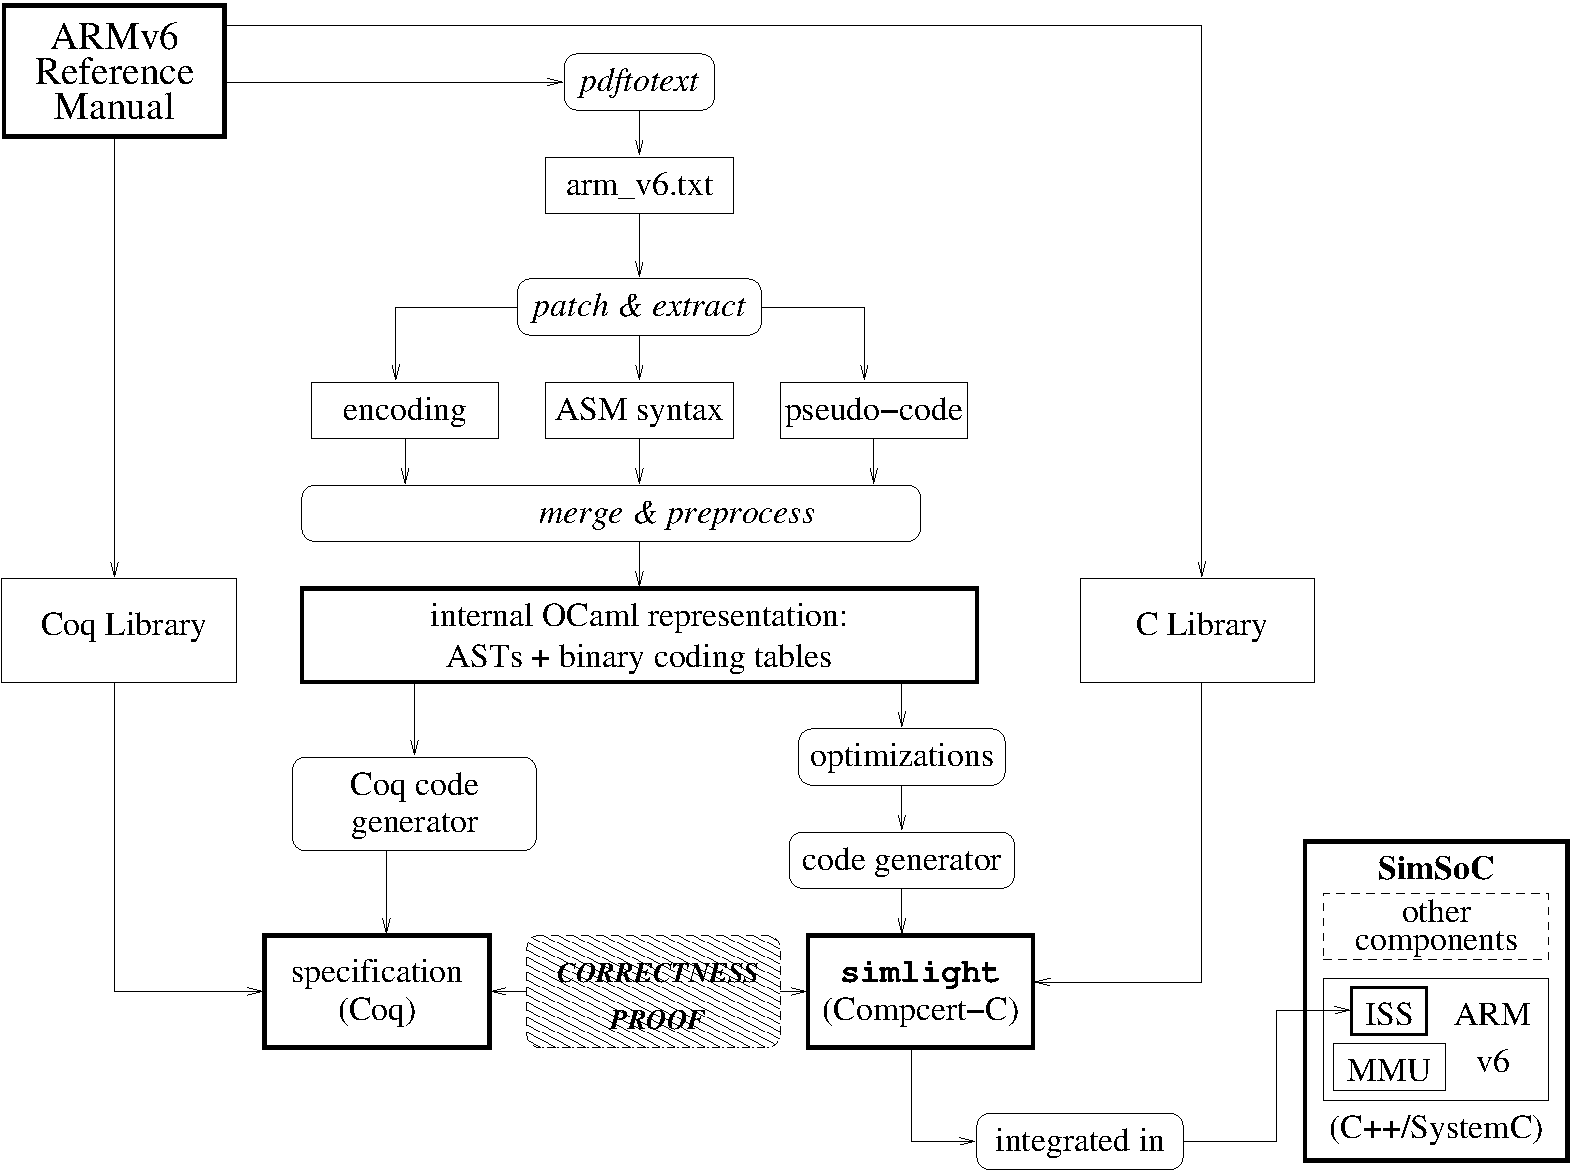
\includegraphics[width=\linewidth]{fig/fullarchi.pdf}
\caption{Overall generation chain}
\label{fig:arch}
\end{figure}

Three kinds of information are extracted for each ARM operation: its
binary encoding format, the corresponding assembly syntax, and its
body, which is an algorithm operating on various data structures
representing the state of an ARM: registers, memory, etc., according
to the fields of the operation considered. This algorithm may call
general purpose functions defined elsewhere in the manual, for which
we provide a \compcert C library to be used by the simulator and a Coq
library defining their semantics. The latter relies on libraries from
the \compcert project that allows us, for instance, to manipulate
32-bits representations of words. The result is a set of abstract
syntax trees (ASTs) and binary coding tables. These ASTs follow the
structure of the (not formally defined) pseudo-code.

In the end, two files are generated: a \compcert C file to be linked
with other components of \simsoc (each instruction can also be
executed in stand-alone mode, for test purposes for instance) and
Coq files representing each instructions in \compcert C AST to be used
for correctness proof.

As the C language accepted by Compcert is a subset of the full ISO C
language, the generator has been constructed such that it only
generates C code in the subset accepted by the compcert compiler.
Nonetheless it can be compiled with other C compilers such as GCC
to obtain better performance. Even though in this case, the resulting
machine code is not guaranteed to be correct (there are well known
GCC optimization bugs...), at least the original C code has been
proven by our technique to be conformant with the ARM semantics.

The ARM V6 code generator not only generates the semantics functions,
it also generates the decoder of binary instructions supported in V6
architectures. This decoder is obtained by compiling the opcodes
information. The generated decoder is probably not optimal in
performance, but as \simsoc uses a cache to store the decoded
instructions, the performance penalty is marginal.

\subsection{Simulator Semantics}

In order to formally reason on the correctness of the simulator, we
need a formal model in Coq of the C implementation of ARM simulator
generated as described above.  It is provided by \compcert, which
defines operational semantics of C formalized in Coq.

As this C program has also as an objective to achieve a high speed
simulator, the generator makes optimizations. In particular, states in
the model of the C implementation are complex not only
because the memory model defined in \compcert is taken into account,
but also because of optimizations and design decisions
targetting efficiency.  In more detail:
\begin{itemize}
\item The C implementation uses a big \emph{struct} to express the ARM
  processor state.  The model of the state is a complex Coq record
  type, including not only data fields but also proofs to guaranteed
  access permission, next block pointer, etc.
\item Transitions are defined with a relational style.  In general,
  the relational style is more flexible but functional definitions
  have some advantages: reasoning steps can be replaced by
  computations; existence and unicity of the result are automatically
  ensured.  However, the functional style is not always convenient or
  even possible.  It is the case here, where the transitions defined
  by the C implementation are relations which happen to be functions.
  This comes first from the operational semantics, which needs to be
  a relation for the sake of generality.  Furthermore in our case, the
  kind of record type mentioned in the previous item is too complex to
  execute calculation with it, so it is more convenient to describe
  the state transformation for memory with a relation.
\item
The global state is based on a complex memory model
with load and store functions that are used for read/write operations.
\end{itemize}


\subsection{Proof}

As a result of the generator described above, we have a C
implementation of the ARM instruction set.  To prove that it is correct
we need a formal specification of that architecture, and prove that
given the initial state of the system, the execution of an instruction
as implemented by a C function results in the same state as the formal
specification.

Ideally the formal specification of the ARM architecture should be
provided by the vendor. But it is not the case, such a formal model is
not available on their web site, hence we had to build one.  As
mentioned in the related work section, we considered using the ARM
formal model defined in \cite{FoxM10}, but it would have required
us to translate all of the C operational semantics as well, which
would not have been error prone, not to mention the effort. So, we
chose to define a formal model of ARM in Coq as well. As Coq models
are executable, we could validate the model with real programs.

The state of the ARMv6 processor defined in the formal model is called
the \emph{abstract state}.  On the other hand, the same state is
represented by the data structure corresponding to C semantics that we
shall call the \emph{concrete state}.  In order to state correctness
theorems we need to relate these two models.  Executing the same
instruction on the two sides will produce a pair of new processor
states which should related by the same correspondance. Informally,
executing the same instruction on a pair of equivalent states will
produce a pair of equivalent states.

Our theorems are then accurately schematized by
Figure~\ref{fig:theoca}, and we want to prove they are equivalent.
The formal proof method is described in detail in
\cite{xiaomu-phd}. We only provide here an outline of the method.

The main strategy is to define a projection from the concrete state to
the abstract state.  On both sides, the execution of an instruction is
described by a state transition.  For the two ISS representations,
``State'' refers to the full description of the system.  We start from
a C memory state corresponding to the abstract state described by
the formal specification.  This correspondance is expressed by a
projection relating the two models of the state.

\begin{figure}
\hfil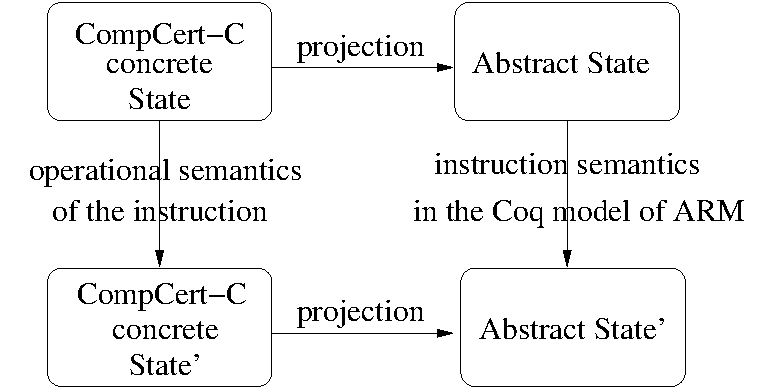
\includegraphics[width=.75\linewidth]{fig/theoremca.pdf}
\caption{Theorem statement for a given ARM instruction}
\label{fig:theoca}
\end{figure}

For the C instruction set, we have a standalone C function for each
ARMv6 instruction.  Each function (instruction) has its own
correctness proof separately.  Every function is composed by its
return type, function parameters, local variables, and the function
body. The function body is a sequence of statements made of
expressions. Let us considering as example the ARM
instruction \texttt{BL Branch and Link}. The generated C code is:
\begin{alltt}\small
void B(struct SLv6_Processor *proc,
       const bool L,
       const SLv6_Condition cond,
       const uint32_t signed_immed_24)\{
  if (ConditionPassed(&proc->cpsr, cond)) \{
    if ((L == 1))
      set_reg(proc,14,
              address_of_next_instruction(proc));
    set_pc_raw(proc,
               reg(proc,15)+
               (SignExtend_30(signed_immed_24) << 2));
 \}
\}
\end{alltt}

The internal \compcert C representation of that C code is equivalent to:

\begin{alltt}\small
Definition fun_internal_B :=
\{|
 fn_return := void;
 fn_params := [
  proc -: `*` typ_SLv6_Processor;
  L -: int8;
  cond -: int32;
  signed_immed_24 -: uint32];
  fn_vars := [];
  fn_body :=\footnotesize
  `if (call (ConditionPassed`:T1)
        E[\&((`*(proc`:T2)`:T3)
         |cpsr`:T4)`:T5;cond`:T6] T7)
  then
   `if ((L`:T7)==(#1`:T6)`:T6)
      then (call (set_reg`:T8)
        E[proc`:T2; #14`:T6;
         (call (address_of_next_instruction`:T9)
                E[proc`:T2] T10)]
           T11)
   else skip;;
    (call (set_pc_raw`:T12)
      E[proc`:T2;
       (call (reg`:T13) E[proc`:T2; #15`:T6] T10)+
        ((call (SignExtend_30`:T14)
         E[signed_immed_24`:T10] T10)
           \<<(#2`:T6)`:T10)`:T10]
      T11)
  else skip \small
 |\}.
\end{alltt}

We need to prove that the operational semantics of that code
correspond to the ARM formal specification.

A significant issue is that C representation introduces a complex
memory model designed for high simulation speed, and we need a mapping
with the formal model. In the \compcert C model, variables are stored
in the memory model.  It maps each variable identifier to its location
and its type, and its value is stored in the associated memory block.
The value associated to a C variable or a parameter of a C function is
obtained by applying (abstract) \texttt{load} to the suitable
reference block in memory.  These two operations are performed when a
function is called, building a local environment \texttt{e} and an
initialized memory state \texttt{m}. The formal model of ARMv6 is
defined as a much simpler functional model and computing the value of
a component can be performed directly.

The proof consists in defining provable projections from the C state
to the formal model to prove their equivalence, as represented in
Figure~\ref{fig:proj}.

\begin{figure}[h]
\hfil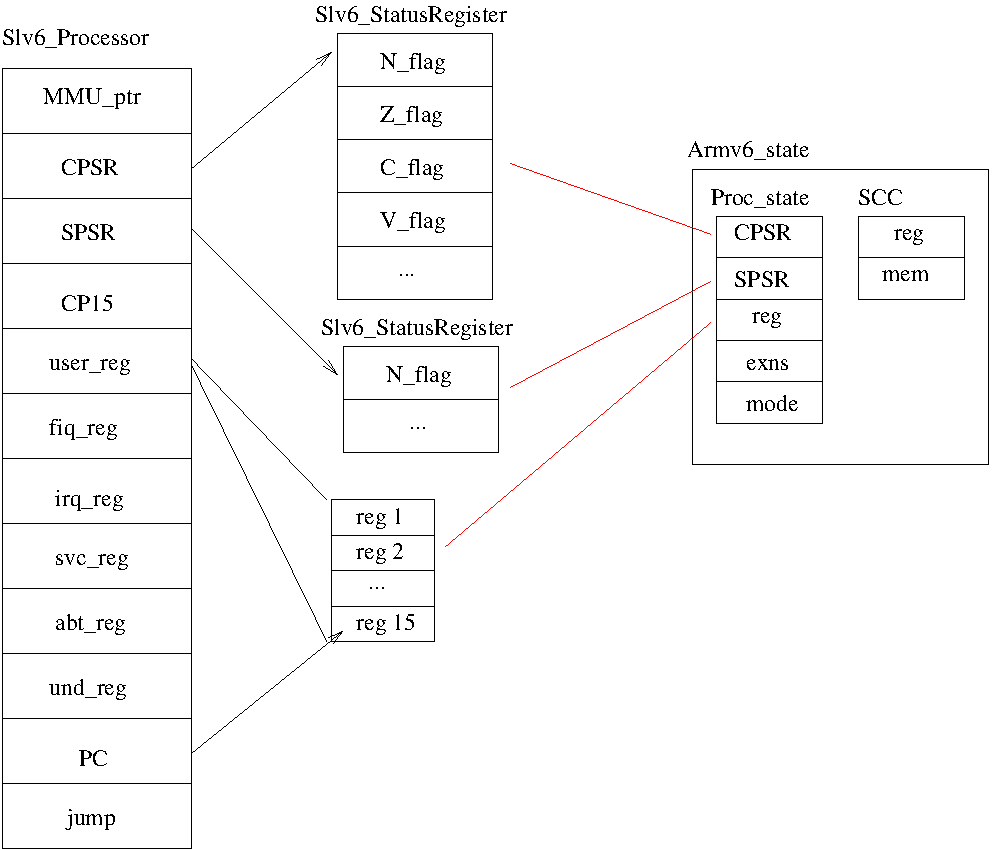
\includegraphics[width=.75\linewidth]{fig/projection.pdf}
\caption{Projection}
\label{fig:proj}
\end{figure}

According to the type of the argument of the
projection, the definitions of projections are different.  For
example, the projection of a register given above performs a case
analysis on a value of type \texttt{register}, whereas the projection
of SPSR depends on the type of exception modes.  We define a specific
projection for each type.  Coq is rich enough to allow us to define a
general projection for all types of elements, using dependent
types. To improve readability of the statement, we chose to
define a projection relation for each instance.

In order to carry out these proofs, we had to prove first a fair
number of lemmas that can also be found in
\cite{xiaomu-phd}. Most of them are related to the semantics of \compcert
C.  Indeed, since the abstract model is defined in a functional style,
many proof steps are reductions. In contrast, the execution of a C
program is provided by inductively defined relationsn from the
operational semantics.  Decomposing the execution step by step
amounts to perform so-called \emph{inversions} on hypotheses relating
concrete memory states according to the operational semantics.  In
practice, a large amount (several dozens) of inversions are performed,
bringing serious issues on space-time consumption and maintenability.
We studied a general solution to this problem, and developed a new
inversion tactics in Coq.

As a result, for each ARM instruction, we have a theorem proving that
the C code simulating an ARM instruction is equivalent to the formal
model of the ARM processor. All of these lemmas and theorems are verified
by the Coq theorem prover.

\section{Towards Certified Program}

We consider here as a simple example the DES cryptographic encryption code.
Once the key has been generated the C code for encrypting a block of data
is straightforward:
\begin{alltt}\small
#define GET_ULONG_BE(n,b,i)
 (n) = ( (unsigned long) (b)[(i)] << 24 )
    | ( (unsigned long) (b)[(i) + 1] << 16)
    | ( (unsigned long) (b)[(i) + 2] <<  8)
    | ( (unsigned long) (b)[(i) + 3]      );

#define DES_IP(X,Y)                               \
    T = ((X >>  4) ^ Y) & 0x0F0F0F0F;
    Y ^= T; X ^= (T <<  4);
    T = ((X >> 16) ^ Y) & 0x0000FFFF;
    Y ^= T; X ^= (T << 16);
    T = ((Y >>  2) ^ X) & 0x33333333;
    X ^= T; Y ^= (T <<  2);
    T = ((Y >>  8) ^ X) & 0x00FF00FF;
    X ^= T; Y ^= (T <<  8);
    Y = ((Y << 1) | (Y >> 31)) & 0xFFFFFFFF;
    T = (X ^ Y) & 0xAAAAAAAA;
    Y ^= T; X ^= T;
    X = ((X << 1) | (X >> 31)) & 0xFFFFFFFF;

#define DES_ROUND(X,Y)
    T = *key++ ^ X;
    Y ^= SB8[ (T      ) & 0x3F ]
       ^  SB6[ (T >>  8) & 0x3F ]
       ^  SB4[ (T >> 16) & 0x3F ]
       ^  SB2[ (T >> 24) & 0x3F ];
    T = *key++ ^ ((X << 28) | (X >> 4));
    Y ^= SB7[ (T      ) & 0x3F ]
         SB5[ (T >>  8) & 0x3F ]
         SB3[ (T >> 16) & 0x3F ]
         SB1[ (T >> 24) & 0x3F ];

void des_crypt_ecb( unsigned long *key,
                    unsigned char input[8],
                    unsigned char output[8] )
{
    int i;
    unsigned long X, Y, T;
    GET_ULONG_BE( X, input, 0 );
    GET_ULONG_BE( Y, input, 4 );
    DES_IP( X, Y );
    for( i = 0; i < 8; i++ )  {
        DES_ROUND( Y, X );
        DES_ROUND( X, Y );
    }
    DES_FP( Y, X );
    PUT_ULONG_BE( Y, output, 0 );
    PUT_ULONG_BE( X, output, 4 );
}
\end{alltt}

Looking at the binary code of that function generated by the compiler,
one may observe that this code contains only 22 different types of ARM
instructions, namely \textbf{ add, and, asr, b, ble, bne, bx, cmp,
  eor, ldm, ldr, ldrb, lsl, lsr, mov, orr, pop, push, str, str, strb,
  sub}.

Given that we have a proof that the machine code generated from C is
correct and a proof of the ARM instructions simulator for these
instructions, we have a proof that the execution of the DES algorithm
on ARM is comformant with the specification.



%%%%%%%%%%%%%%%%%%%%%%%%%%%%%%%%%%%%%%%%%%%%%%%%%%%%%%%%%%%%%%%%%
\section{Conclusion}
\label{conclusion}
We have constructed a tool chain that makes it possible to certify
that the execution of a program is conformant with the formal
definition of the algorithm, by leveraging off from three existing tools
namely, Compcert-C, Coq and SimSoc, to which we have added a proven
generated simulator of the ARM instruction set.

Although we have considered a small example in the paper, there is no
limit on the size of the C code that can be certified as long as
the instruction set has been certified.

We acknowledge however that there are two weak points in this chain,
the C code taken as example has not been generated from a formal specification
but there are now several frameworks that generate code from formal
specification, and mostly the fact that the hardware vendors do not
provide formal semantics of their instruction set. As these are
unavailable we had to define one that we have validated manually
but not formally. If the vendors would make public formal specification
of the architecture, then our toolchain would becomes verified.



%%%%%%%%%%%%%%%%%%%%%%%%%%%%%%%%%%%%%%%%%%%%%%%%%%%%%%%%%%%%%%%%%%
\section*{Acknowledgments}

This work has been supported jointly by INRIA, Tsinghua University,
Shenzhen Institutes of Advanced Technology, Chinese Academy of
Sciences.

%%%%%%%%%%%%%%%%%%%%%%%%%%%%%%%%%%%%%%%%%%%%%%%%%%%%%%%%%%%%%%%%%%

\bibliographystyle{IEEEtran}

%\bibliographystyle{abbrv}
% End the column at reference X to balance 2 columns
%\IEEEtriggeratref{13}
%\bibliography{IEEEabrv,references.bib}
\bibliography{references}

\end{document}
